\documentclass[11pt,a4paper]{book}
\textwidth 170 mm
\textheight 250 mm
\topmargin -15 mm
\oddsidemargin -5 mm
\evensidemargin -5 mm

\newcounter{ProblemNo}
\setcounter{ProblemNo}{0}
\def\tempID{0}
%\def\UndAns{} %% <-------------- Uncomment in final version!!
\def\UndAns{\underline}
\def\UndAns{\underline}
\newcommand{\ZOdg}[1]{}
\def\text{}
%\def\dfrac{\displaystyle\frac}

\usepackage{amsfonts,amssymb,amsmath}
\usepackage{graphicx}
\DeclareGraphicsExtensions{.pdf,.PDF,.png,.PNG} % prefer pdf to png
\usepackage{etoolbox}
\usepackage{sidepicture}
\newcommand{\problemID}[3]{\def\tempID{#1 (#3)}\ignorespacesafterend}
%\newcommand{\problemID}[3]{\def\tempID{#1}\noindent{\bf #1, #2}\par}
%\newcommand{\problemID}[3]{\def\tempID{#3: \##1}\par}
%\newcommand{\problemRating}[3]{{\bf #1, #2, #3}\par}
%\newcommand{\problemID}[3]{\def\tempID{\# #1}\par}
%\newcommand{\problemRating}[3]{}
%\newcommand{\xProblem}[8]{#1\par (A) #2\quad (B) #3\quad  (C) #4\quad  (D) #5\quad (E) #6\par Correct: #7\bigskip\bigskip\par }

%\usepackage{xcolor}
%\usepackage{everypage}
%\usepackage[absolute]{textpos}
%\usepackage{rotating}
%\AddEverypageHook{\begin{textblock*}{2.5cm}(0.7cm,5cm)\begin{turn}{90}{\color{red}\Huge\sc Solutions included - do not use for contest}\end{turn}\end{textblock*}}

\newcommand{\Problem}[9]
{%\newpage
%\noindent\addtocounter{ProblemNo}{1}{\bf\arabic{ProblemNo}.\hspace{3pt}~}%
\noindent\addtocounter{ProblemNo}{1}{\bf\tempID.\hspace{3pt}~}%
\edef\answer{{#7}}\def\SettingMode{#8}%
\def\VLine{\vrule height14pt width0pt\quad}#1\nopagebreak\vspace{1ex}\newline%
\VLine\expandafter\ifstrequal\answer{A}{\UndAns{(\rlap{\bf A}\phantom{\bf C})}\ZOdg{A}}{(\rlap{\bf A}\phantom{\bf C})}\nolinebreak\hspace{3pt}%
\ifnum\SettingMode=3{#2}\else\rlap{#2}\fi\quad\ifnum\SettingMode=3\newline\VLine\else\hfil\fi%
\expandafter\ifstrequal\answer{B}{\UndAns{(\rlap{\bf B}\phantom{\bf C})}\ZOdg{B}}{(\rlap{\bf B}\phantom{\bf C})}\nolinebreak\hspace{3pt}%
\ifnum\SettingMode=3{#3}\else\rlap{#3}\fi\quad\ifnum\SettingMode=2\newline\VLine\else\ifnum\SettingMode=3\newline\VLine\else\ifnum\SettingMode=6{\phantom{({\bf C})}\quad\hspace{6pt}\hfil\hfil\newline\VLine}\else\hfil\fi\fi\fi%
\expandafter\ifstrequal\answer{C}{\UndAns{(\rlap{\bf C}\phantom{\bf C})}\ZOdg{C}}{({\bf C})}\nolinebreak\hspace{3pt}%
\ifnum\SettingMode=3{#4}\else\rlap{#4}\fi\quad\ifodd\SettingMode\newline\VLine\else\hfil\fi%
\expandafter\ifstrequal\answer{D}{\UndAns{(\rlap{\bf D}\phantom{\bf C})}\ZOdg{D}}{(\rlap{\bf D}\phantom{\bf C})}\nolinebreak\hspace{3pt}%
\ifnum\SettingMode=3{#5}\else\rlap{#5}\fi\quad\ifnum\SettingMode>1\ifnum\SettingMode<6\newline\VLine\else\hfil\fi\else\hfil\fi%
\expandafter\ifstrequal\answer{E}{\UndAns{(\rlap{\bf E}\phantom{\bf C})}\ZOdg{E}}{(\rlap{\bf E}\phantom{\bf C})}\nolinebreak\hspace{3pt}%
\ifnum\SettingMode=3{#6}\else\rlap{#6}\fi\quad\ifnum\SettingMode=1\hfil\phantom{({\bf C})}\fi\hspace{3pt}\hfil\par\vspace{2ex}\par\noindent{\sc Solution: }#9\bigskip}


\def\TheHead{Student Finalized}
\makeatletter
\def\ps@pKSF{
\def\@oddfoot{\hfill{\rm \thepage}\hfill}\def\@evenfoot{\hfill{\rm \thepage}\hfill}
\def\@oddhead{\hfill{\em \TheHead}\hfill}\def\@evenhead{\hfill{\em \TheHead}\hfill}
}
\makeatother 
\pagestyle{pKSF}

\begin{document}

\noindent{\large\bf Student}\bigskip

\noindent\fbox{3 points}\bigskip

\NSidePictureEPS[scale=0.7]{S01-7}{\problemID{1}{20287}{Slovenia}%
\problemRating{S}{3}{L}%
\Problem{A pattern is made of equal pentagons. Which of the tiles below, when placed in the central hole, will form a self-intersecting loop?}
{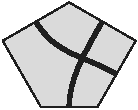
\includegraphics[scale=0.7]{S01-1}}{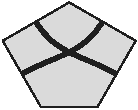
\includegraphics[scale=0.7]{S01-2}}{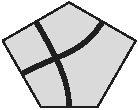
\includegraphics[scale=0.7]{S01-3}}{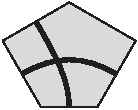
\includegraphics[scale=0.7]{S01-4}}{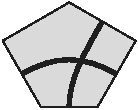
\includegraphics[scale=0.7]{S01-5}}
{C}{1}
{Note that all tiles are rotated by $180^\circ$. 
No other rotation can make the tile fit as the pentagonal tile has exactly two right angles.
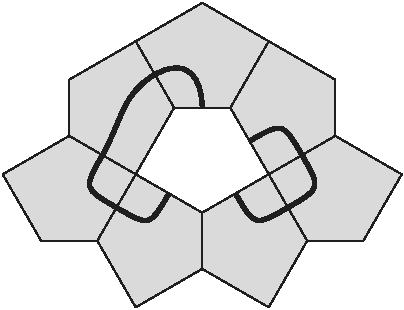
\includegraphics[scale=0.7]{S01-6}}}

\problemID{2}{20288}{United Kingdom}%
\problemRating{S}{3}{N}%
\Problem{Which of these integers is two less than a multiple of ten, two more than a square, and two times a prime?}
{$78$}{$58$}{$38$}{$18$}{$6$}
{C}{0}
{All the given options but (E) are two less than a multiple of ten. However, both $38$ and $18$ are two more than a square ($36$ and $16$) but only $38$ is two times a prime ($2 \times19$).  Hence the answer is $38$.}

\NSidePictureEPS[yoffset=-3.5ex]{S03-1}{\problemID{3}{20289}{Germany}%
\problemRating{S}{3}{G}%
\Problem{A young kangaroo cut a pizza into six equal slices.
After eating one slice, he arranged the remaining slices with equal gaps between slices.
What size is the angle of each gap?}
{$5^\circ$}{$8^\circ$}{$9^\circ$}{$10^\circ$}{$12^\circ$}
{E}{1}
{The sum of the angles of all 5 gaps is $\dfrac{360^\circ}{6} = 60^\circ$. Hence, the angle of each gap is $\dfrac{60^\circ}{5} = 12^\circ$.}}

\problemID{4}{20290}{Finland}%
\problemRating{S}{3}{A}%
\Problem{Juuso has an unusual habit of drawing the $xy$-plane with the positive coordinate axes pointing left and down.
What would the graph of the equation $y=x+1$ look like in a coordinate system drawn by Juuso?}
{\includegraphics{S04-1}}{\includegraphics{S04-2}}{\includegraphics{S04-3}}{\includegraphics{S04-4}}{\includegraphics{S04-5}}
{D}{0}
{The graph should pass the $y$-coordinate at $1$ and $y$ should increase as the $x$-coordinate increases, so the correct answer is D.}

\problemID{5}{20291}{Germany}%
\problemRating{S}{3}{N}%
\Problem{Kaito has manipulated a die.
The probabilities of rolling a 2, 3, 4 or 5 are still $\dfrac{1}{6}$ each, but the probability of rolling a 6 is twice the probability of rolling a 1.
What is the probability of rolling a 6?}
{$\dfrac{1}{4}$}{$\dfrac{1}{6}$}{$\dfrac{7}{36}$}{$\dfrac{2}{9}$}{$\dfrac{5}{18}$}
{D}{0}
{We have $p(1) + p(6) = 1 - 4 \cdot \dfrac{1}{6} = \dfrac{1}{3}$ and $p(6) = 2 \cdot p(1)$.
So we get $p(6) = \dfrac{1}{3} - p(1) = \dfrac{1}{3} - \dfrac{p(6)}{2}$.
Therefore, $p(6) = \dfrac{1}{3} \cdot \dfrac{2}{3} = \dfrac{2}{9}$.}

\problemID{6}{20292}{Russia}%
\problemRating{S}{3}{N}%
\Problem{Which of the expressions below has the same value as $16^{15} + 16^{15} + 16^{15} + 16^{15}$?}
{$16^{19}$}{$4^{31}$}{$4^{60}$}{$16^{60}$}{$4^{122}$}
{B}{0}
{Notice that $16=4^{2}$ and write the expression as follows:
$16^{15} + 16^{15} + 16^{15} + 16^{15} = 4 \cdot (4^{2})^{15} = 4 \cdot 4^{30} = 4^{31}$}

\problemID{7}{20293}{Finland}%
\problemRating{S}{3}{L}%
\Problem{Beaver wishes to color the squares and triangles of the following figure so that no two neighbouring figures, even those sharing a single vertex, are the same color. \newline
\centerline{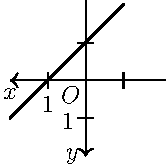
\includegraphics{S07-1}}\newline
What is the least number of colors needed?}
{$3$}{$4$}{$5$}{$6$}{$7$}
{C}{0}
{There are points where five figures meet, so at least five colours are needed. Five is also enough, as seen in this figure. \newline
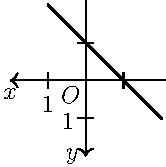
\includegraphics{S07-2}}

\problemID{8}{20294}{China}%
\problemRating{S}{3}{L}%
\Problem{There are $6$ glasses on a table with their open ends up. In any one move, we turn over exactly $4$ of them. What is the least number of moves required to have all glasses upside down?}
{$2$}{$3$}{$4$}{$5$}{$6$}
{B}{0}
{Whatever the first move, we will have 4 glasses down and 2 up.  There is no 2nd move which will have all the glasses down.  However we can  move D(DDDU)U to D(UUUD)U which leaves 4 glasses pointing up which we can turn over in the third move. Hence the answer is $3$.}

\problemID{9}{20295}{Greece}%
\problemRating{S}{3}{N}%
\Problem{A student started with the number $1$ and multiplied it by either $6$ or $10$. He then multiplied the result by either $6$ or $10$, and continued this procedure many times. Which of the following cannot be one of the numbers he obtained?}
{$2^{100} 3^{20}5^{80}$  }{$2^{90} 3^{20}5^{80}$ }{$2^{90} 3^{20}5^{70}$ }{$2^{110} 3^{80}5^{30}$  }{$2^{50} 5^{50}$ }
{B}{1}
{If he used the factor $6$ $N$ times and the factor $10$ $M$ times, the number he would get is of the form $(2\cdot 3)^N(2\cdot 5)^M= 2^{N+M}3^N5^M$. Observe that the exponent of $2$ is equal to the sum of the exponents of $3$ and of $5$. Of the numbers given the only one that fails this is B, as $90 \ne 20+80$.}

\NSidePictureEPS{S10-1}{\problemID{10}{20296}{Greece}%
\problemRating{S}{3}{A}%
\Problem{A black trail and a grey trail cross a park, as shown. Each trail divides the park into two regions of equal area.  Which of the following must be true about the areas $A$, $B$ and $C$?}
{$A=C$}{$B=A+C$ }{$ B=\dfrac{1}{2}(A+C)$   }{$ B=\dfrac{2}{3}(A+C) $ }{  $ B=\dfrac{3}{5}(A+C) $ }
{B}{1}
{To the left of the black trail, we have $D+B$ is half the park.  To the left of the grey trail, we have $D+A+C$ is half the park.  Equating these, we see that $B=A+C$.\newline
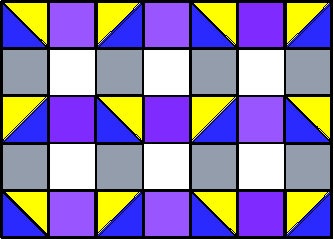
\includegraphics{S10-2}}}

\noindent\fbox{4 points}\bigskip

\problemID{11}{20297}{Finland}%
\problemRating{S}{4}{L}%
\Problem{Exactly one of these statements about a certain positive integer $n$ is true. Which statement is true?}
{$n$ is divisible by 3}{$n$ is divisible by 6}{$n$ is odd}{$n = 2$}{$n$ is prime}
{C}{1}
{D cannot be true since E would also be true. 
B cannot be true because A would also be true. 
Since n is not 2, if E were true, C would also be true, so E cannot be true.
The true statement is either A or C. If A is true, then C is not, but then B would be true. So A cannot be true either, and the answer must be C.
The number $n$ must be some odd number that is not divisible by 3 nor is it prime, for example $n = 25$.}

\newpage\problemID{12}{20298}{Greece}%
\problemRating{S}{4}{G}%
\Problem{A triangular pyramid $ABCD$ has sides of length $5$, $6$, $7$, $8$, $9$ and $10$. The points $M$, $N$, $P$, $Q$, $R$ and $S$ are the midpoints of the edges of the pyramid, as shown. \newline
\centerline{\includegraphics{S12-1}}
\newline
What is the perimeter of the closed hexagonal line $MNPQRSM$?}
{$19$}{$20$}{$21$}{$22$}{$23$}
{C}{0}
{$MN$ is half of $BC$. In fact each side of the closed hexagonal line is half a corresponding parallel edge. So the perimeter of the hexagon (starting from the segment $MN$) is $\dfrac{1}{2}(10+5+6+7+8+6)=21$.}

\NSidePictureEPS{S13-2}{\problemID{13}{20299}{China}%
\problemRating{S}{4}{G}%
\Problem{A quadrilateral $ABCD$ has two right angles at $B$ and $C$, where $AB=4, BC=8$ and $CD=2$. Point $X$ lies on $BC$. What is the minimum value of $AX+DX$?}
{$9\sqrt{2}$}{12}{13}{10}{None of the previous}
{D}{2}
{If we extend the line $AB$ to the point $Y$ , where $AB=BY$, connect $YD$ which crosses the side $BC$ at point $X$, then connect $AX$. From the graph, we know that $AX=YX$, the minimum value of $AX+DX$ is $YD$.\newline
$YD=\sqrt{BC^2+(BY+CD)^2}=\sqrt{8^2+6^2}=10$\newline
\includegraphics{S13-3}}}

\problemID{14}{20300}{Austria}%
\problemRating{S}{4}{G}%
\Problem{John has a number of all black or all white unit cubes and wants to build a $3\times 3\times 3$ cube using $27$ of them. He wants the surface to be exactly half black and half white. What is the smallest number of black cubes he can use?}
{$14$}{$13$}{$12$}{$11$}{None of the previous}
{E}{4}
{None of the numbers in the answers. In fact  the smallest number is $10$. There are $9$ small squares showing on each of the $6$ faces of the large cube, for a total of $54$. In order for $27$ of these to be black, he can put a black cube in each of the $8$ corners ($3\times 8 = 24$ small black squares) and one each in a central edge spot ($2$ black squares) and a central face spot (one black square).}

\NSidePictureEPS[yoffset=-7.5ex,scale=0.4]{S15-2}{\problemID{15}{20301}{Russia}%
\problemRating{S}{4}{G}%
\Problem{A diagonal, a semicircle and a quadrant are drawn in a square of side 6 cm. What is the area, in cm$^2$, of the shaded part?}
{$9$}{$3\pi$}{$6\pi-9$}{$10\pi/3$}{$12$}
{A}{0}
{Notice that part 1 coincides with the same part on the right. Combining of 1 and 2 coincides with the same part on the top: \newline
\includegraphics[scale=0.4]{S15-1} \newline
Thus all painted part coincides with the quarter of the square area. Then its area is $6^{2} \div 4 = 36 \div 4 = 9$.}}

\NSidePictureEPS[xlines=2]{S16-2}{\problemID{16}{20302}{Greece}%
\problemRating{S}{4}{G}%
\Problem{The figure shows four squares. The smaller ones have side lengths $a$, $b$ and $c$. The vertices $A$ and $C$ of two of the smaller squares coincide with two diagonally opposite vertices of the large square. The vertex $B$ of the third small square is on the side of the large one. Which of the following expressions represents the side length of the largest square?}
{$\dfrac {1}{2}(a+b+c) $}{ $\sqrt {a^2+b^2+c^2}$}{$\sqrt {(a+b)^2+c^2}$  }{ $\sqrt {(b-a)^2+c^2}$    }{  $\sqrt {a^2+ab + b^2+c^2}$  }
{C}{1}
{It is easy to see that the two shaded right angled triangles are equal (hypotenuses equal and one acute angle equal). Then by Pythagoras on one of them we get $x^2=(a+b)^2+c^2$. 
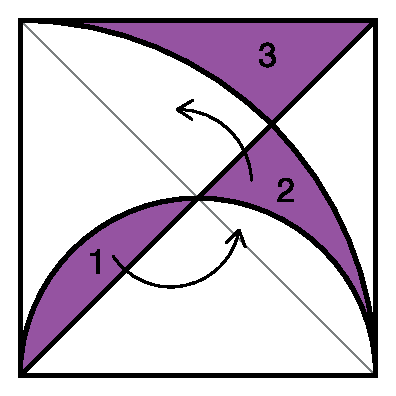
\includegraphics{S16-1}}}

\problemID{17}{20303}{United Kingdom}%
\problemRating{S}{4}{A}%
\Problem{We have two positive numbers $p$ and $q$, with $p<q$. Which of these expressions is the largest?}
{$\dfrac{p+3q}4$}{$\dfrac{p+2q}3$}{$\dfrac{p+q}2$}{$\dfrac{2p+q}3$}{$\dfrac{3p+q}4$}
{A}{0}
{First write all the options as expressions with a common denominator of 12 to give $\dfrac{3p+9q}{12}$, $\dfrac{4p+8q}{12}$, $\dfrac{6p+6q}{12}$, $\dfrac{8p+4q}{12}$ and $\dfrac{9p+3q}{12}$.  Since we are told that $p < q$ and the sum of the coefficients of $p$ and $q$ in each expression is the same, the largest expression is the one with the largest coefficient of $q$.  Therefore the largest expression is $\dfrac{3p+9q}{12}$ or $\dfrac{p+3q}4$.
\newline
Alternatively, we can observe that each of the expressions is a weighted average of $p$ and $q$.  As $p<q$, the expression with the greatest proportion of $q$ will be the largest, which is A.}

\problemID{18}{20304}{Russia}%
\problemRating{S}{4}{N}%
\Problem{How many three-digit numbers are there that contain at least one of the digits $1$, $2$ or $3$?}
{$27$}{$147$}{$441$}{$557$}{$606$}
{E}{0}
{There are $900$ three-digit numbers in total. Let's calculate how many of them do not contain $1$, $2$ or $3$. The first digit of such a number could be $4$, $5$, $6$, $7$, $8$ or $9$, giving 6 options. For each of the second and third digits, there are 7 options. So there are $6 \cdot 7 \cdot 7 = 294$ numbers. Therefore there are $900 - 294 = 606$ numbers that contain at least one of digits $1$, $2$ or $3$.}

\problemID{19}{20305}{Australia}%
\problemRating{S}{4}{A}%
\Problem{I write down a 4-digit non-zero number $N=\overline{pqrs}$. When I place a decimal point between
 the $q$ and the $r$, I find that the resulting number $\overline{pq.rs}$ is the
 average of the two-digit numbers $\overline{pq}$ and $\overline{rs}$.
 
 What is the sum of the digits of $N$?}
{$14$}{$18$}{$21$}{$25$}{$27$}
{B}{0}
{We observe that $pq$ and $rs$ are whole numbers, so their average must end in .00 or .50.  However, if $rs =0$, the average of $pq$ and $rs$ cannot be more than $pq$, so $rs$ is $50$.  This means that $pq$ must be $49$ and the average is $49.50$.  Hence the original number is $4950$ with digital sum $18$.}

\problemID{20}{20306}{Australia}%
\problemRating{S}{4}{A}%
\Problem{Two candles of equal length start burning at the same time.
 One of the candles will burn down in $4$ hours, the other in $5$ hours, each at their own constant rate.
 How many hours will they have to burn before one candle is $3$ times
 the length of the other?}
{$\dfrac{40}{11}$}{$\dfrac{45}{12}$}{$\dfrac{63}{20}$}{$3$}{$\dfrac{47}{14}$}
{A}{0}
{Let the initial length of each candle be $l$. Let candle A be the faster burning
 candle, completely burning in 4 hours, and let B be the slower burning
 candle. After $t$ hours the lengths of the candles are

 A: $l(1-t/4)$
 B: $l(1-t/5)$

 We need to find $t$ such that
 length of B $= 3 \times$ length of A

 \begin{align*}
 l(1-t/5)&=3l(1-t/4)\\
 20-4t&=60-15t\\
 11t&=40\\
 t&=40/11
 \end{align*}}

\noindent\fbox{5 points}\bigskip

\problemID{21}{20307}{Czech Republic}%
\problemRating{S}{5}{N}%
\Problem{Andre has six cards with one number written on each side of each card. The pairs of numbers on the cards are  $(5,12), (3,11), (0,16), (7,8), (4,14)$ and $(9,10)$.\newline
The cards can be placed in any order in the blank spaces of the figure.\newline
\centerline{\includegraphics{S21-1}}\newline
What is the smallest result he can get?}
{$-23$}{$-24$}{$-25$}{$-26$}{$-27$}
{D}{0}
{Let the numbers $a, \,\, A, \,\, a < A,$ be written on one card and the numbers $b, \,\, B, \,\, b < B,$ be written on another, and let be $a + A < b + B$. Then we observe that $a - B < b - A$. So we select the three cards with the smallest totals on both sides of the cards and put their smaller numbers to the $+$ signs. Then we put the other three cards with their bigger numbers to the $-$ signs .}

\problemID{22}{20308}{Australia}%
\problemRating{S}{5}{A}%
\Problem{Kangaroo solves the equation $ax^2 + bx + c = 0$, and Beaver solves the equation $bx^2 + ax + c = 0$, where $a, b, c$ are pairwise distinct non-zero integers. It turns out that the equations share a solution. Which of the following must be true?}
{The common solution must be $0$.}{The quadratic equation $ax^2 + bx + c = 0$ has exactly one real solution.}{$a>0$}{$b<0$}{$a+b+c=0$}
{E}{3}
{If the common solution is $r$, then we have $ar^2 + br + c = br^2 +
 ar + c$, which leads to $(a-b)r(r-1) = 0$. Since $a \neq b$ and $c
 \neq 0$, it must be the case that $a-b \neq 0$ and $r \neq 0$.
 Hence, we deduce that the common solution is $r = 1$, which implies
 that $a + b + c = 0$.}

\NSidePictureEPS[yoffset=-3.5ex]{S23-2}{\problemID{23}{20309}{Australia}%
\problemRating{S}{5}{G}%
\Problem{I have a strip of paper that is $12\,$cm long and $2\,$cm wide.
I make a crease across it at $45^\circ$ and then fold it, so that the two parts of the strip are aligned in a right angle, as shown.\newline
What is the smallest possible length, in cm, of $XY$?}
{$6\sqrt{2}$}{$7\sqrt{2}$}{$10$}{$8$}{$6+\sqrt{2}$}
{B}{0}
{\includegraphics{S23-1}
Consider the right-angled triangle $XZY$. The sides $XZ$ and $ZY$ add to 14.  We want to minimise the hypotenuse $XY$ of this triangle and this will occur when the triangle is isosceles. Hence the answer is $7\sqrt2$.}}

\problemID{24}{20310}{Australia}%
\problemRating{S}{5}{N}%
\Problem{Rasika has several unbiased 12-sided dice,
 each with faces labelled $1$ to $12$. When rolling all the dice at once,  the probability of rolling a $12$
 exactly once is equal to the probability of rolling no $12$s. How many
 dice does Rasika have?}
{$8$}{$9$}{$10$}{$11$}{$12$}
{D}{0}
{Suppose she is using $n$ dice. Rolling exactly one 12 amounts to
 choosing one of the $n$ dice to show 12 and all $n-1$ others to
 not show 12, which happens with probability
 $n\times\frac1{12}\times\left(\frac{11}{12}\right)^{n-1}$. On the
 other hand, rolling no 12s has probability
 $\left(\frac{11}{12}\right)^n$.

 Setting these probabilities equal and cancelling a common factor of
 $\left(\frac{11}{12}\right)^{n-1}$, we see that
 $\frac{n}{12}=\frac{11}{12}$, so $n=11$}

\problemID{25}{20311}{Greece}%
\problemRating{S}{5}{A}%
\Problem{A polynomial $p(x)$ satisfies the relation $p(x+1)= x^2-x+2p(6)$ for every real $x$. What is the sum of the coefficients of $p$?}
{$-40$}{$-6$}{$12$}{$40$}{None of the previous }
{A}{4}
{Putting $x=5$ we get $p(6)= 25-5+2p(6)$ so that $p(6) = -20$. Now the given equation becomes $p(x+1)= x^2 -x - 2\times 20= x^2 -x - 40\, (*)$. A quick way to find the sum of the coefficients of $p$ is to observe that it is $p(1)$ (this is true for all polynomials). So putting $x=0$ we get $p(1)= -40$.}

\problemID{26}{20312}{Australia}%
\problemRating{S}{5}{A}%
\Problem{The values of $x,y$ and $z$ satisfy $2^x=3$, $2^y=7$ and $6^z=7$.  Which of the following gives the relationship between $x,y$ and $z$?}
{$z=\dfrac y{1+x}$}{$z=\dfrac x{y}+1$}{$z=\dfrac yx-1$}{$z=\dfrac x{y-1}$}{$z=y-\dfrac1x$}
{A}{0}
{Using various index laws, we have
 \[7=6^z=(2\times3)^z=2^z\times3^z=2^z\times(2^x)^z=2^z\times2^{xz}=2^{z+xz}=2^{z(1+x)}.\]
 But also $2^y=7$, so $y=z(1+x)$ and therefore $z=\dfrac y{1+x}$}

\problemID{27}{20313}{Greece}%
\problemRating{S}{5}{L}%
\Problem{A strip of paper consists of eight squares. Initially each square contains the number 0. In every move ,we chose 4 consecutive squares and add one to each of the numbers in those squares. The figure on the right shows the outcome after a number of moves but unfortunately some ink is covering some of the squares. What number is written on the square with the question mark?    
\centerline{\includegraphics{S27-1}}}
{24}{30}{36}{48}{None of the previous}
{A}{4}
{After $a$ operations with the first four squares, $b$ with the second run of four squares, etc, we will end up in a situation as in the figure. 

\includegraphics{S27-2}
\newline
From observing squares $B$ and $C$, we see that $c=12$.  Now look at squares $F$ and $G$.  The difference between them is $c$, so $G =36-12=24$.
\newline
If we want an example to show that the situation is attainable, we may take $a=17, b=13, c=12, d=10$ and $e=14$.}

\problemID{28}{20314}{Greece}%
\problemRating{S}{5}{A}%
\Problem{A function $f \colon \mathbb R \longrightarrow \mathbb R$ satisfies $f(20-x)=f(22+x)$ for all real $x$. It is known that $f$ has exactly two roots. What is the sum of these two roots?}
{$-1$}{$20$}{$21$}{$22$}{None of the previous}
{E}{4}
{If $a$ is one of the roots we can choose $x$ so that $20-x=a$, that is, $x=20-a$.  This gives $f(a)= f(42-a)$. So $42-a$ is also a root. Hence, the sum of the roots is $a+(42-a)= 42$. 
\newline Note that $42-a$ is definitely a different root because suppose $a=42-a$, so $a=21$. If $b$ is the second root mentioned in the problem, so $b \ne 21$, then by the above $42-b$ is also a root. But as $b \ne 42 -b $ (because $b\ne 21$), the equation would have three distinct roots, $a, b, 42-b$ contrary to assumption. 
Hence $a$ and $42-a$ are distinct. 
\newline
Another way to solve the problem is to use symmetry: The given equation can be written as $f(21-t)=f(21+t)$. So the line $x=21$ is an axis of symmetry of the graph of $f$.  The result follows from this.}

\problemID{29}{20315}{Australia}%
\problemRating{S}{5}{G}%
\Problem{Twelve points are equally spaced on a circle.  How many triangles containing a $45^\circ$ angle can be formed by choosing three of these points?}
{$48$}{$60$}{$72$}{$84$}{$96$}
{D}{0}
{An angle of $45^\circ$ is created by a line subtended by two points
  spaced three apart. For any given base arc three points apart, there
  are 8 positions for the third vertex of the triangle.  So we have $12
  \times 8=96$ possible triangles.  However, any isosceles triangles
  will be counted twice and there are 12 of these, so the total of
  different triangles is $96 - 12 = 84$}

\problemID{30}{20316}{Switzerland}%
\problemRating{S}{5}{N}%
\Problem{A special four-digit number $\overline{abcd}$ satisfies the equation $\overline{abcd} = a^{a}+b^b+c^c+d^d$.
What is the value of $a$?}
{$2$}{$3$}{$4$}{$5$}{$6$}
{B}{0}
{Estimation shows that $6^6 > 10000$, $4^4=256$ so we cannot have a 6 or more as one of the digits, but without the 5 the right hand side won't be larger than 1000, so among $a,b,c,d$ there should be exactly one 5, that makes $a=3$ since $5^5=3125$.
The special number is $3435$.}


\end{document}